\documentclass[letterpaper]{uitproposal}
\usepackage[utf8]{vietnam}
\usepackage{placeins}
\usepackage{amsfonts}
\usepackage{textcomp}
\usepackage{dblfloatfix}
\usepackage{subfig}
\usepackage{lineno}
\usepackage{amssymb}
\usepackage{tabularx,booktabs}
\usepackage{longtable, lipsum}
\usepackage{amsmath}
\usepackage{mathtools}
\usepackage{graphicx}
\usepackage{lscape}
\usepackage{caption}
\usepackage{hyperref}
\usepackage[sorting=nyt]{biblatex}
\usepackage{mathtools}
\usepackage{lipsum}
\usepackage{fancyhdr}
\usepackage{titlesec}
\usepackage{makecell}
\usepackage{lipsum}
\usepackage{etoolbox}

% Confif variable

\title{Latex template for master student at UIT-VNUHCM}
\vntitle{Biểu mẫu latex dành cho học viên cao học tại Trường đại học công nghệ thông tin, Đại học quốc gia thành phố Hồ Chí Minh}
\proposaltype{Luận văn thạc sĩ ngành An toàn thông tin}
\supervisorname{GS. TS. Copilot with GPT-4}
\studentname{Nguyễn Hồng Sơn}


% Config reference
\addbibresource{references/chapter-1.bib}
\addbibresource{references/chapter-2.bib}


% Begin document

\begin{document}
\headerbox
\vnproposalheader
\vnproposalname
\clearpage
\counterwithin{equation}{section}
\counterwithin{table}{section}
\counterwithin{figure}{section}
\setcounter{secnumdepth}{3}


\pagestyle{fancy}
\fancyhf{}

\fancyfoot[C]{\thepage}

\if @twoside
  \fancyhead[EL,OR]{\bfseries\nouppercase\rightmark}
\else
  \fancyhead[R]{\bfseries\nouppercase\rightmark}
\fi

\section{Tóm tắt đề tài}
\label{summary}

Trong báo cáo này, học viên trình bày một số nội dung cơ bản, phương pháp sử dụng và một số ví dụ của các thư viện được áp dụng trong bài toán phát hiện đối tượng. Các nội dung được trình bày sẽ bao gồm nhưng không giới hạn bởi khái niệm, phương pháp huấn luyện, phương pháp dự đoán, các cài đặt và các nội dung khác. Do giới hạn về tài nguyên và thời gian, các nội dung training trong các công cụ không được đề cập trong báo cáo này. Khi so sánh về hiệu suất huấn luyện của các công cụ, các kết quả từ các nghiên cứu đã được công bố sẽ được sử dụng thay vì kết quả thực nghiệm của học viên.

Phần \ref{sec:introduction} giới thiệu tổng quan về bài toán phát hiện đối tượng và các thư viện TensorFlow Object Detection API, Detectron2, MXNet GluonCV, MMDetectio cùng các ví dụ của chúng. Phần \ref{sec:compare} so sánh các thư viện với nhau và đưa ra kết luận. Cuối cùng là tài liệu tham khảo
\section{Giới thiệu}
\label{sec:introduction}

\subsection{Tổng quan về bài toán phát hiện đối tượng}

Phát hiện đối tượng (Object Detection) được coi là một trong những lĩnh vực quan trọng nhất trong nghiên cứu máy học nói chung và xử lý ánh nói riêng. Các mô hình phát hiện đối tượng được training nhằm nhận diện các đối tượng, phát hiện đối tượng là gì trong các hình ảnh hoặc video.

Convolutional Neural Network(CNN) là một kiến trúc học sâu lấy cảm hứng từ nhận thức trực quan của sinh vật. Năm 1980 Kunihiko Fukushima\cite{fukushima1980self} đề xuất neocognitron , có thể coi là tiền thân của CNN. Kể từ đó, nhiều nghiên cứu mới về CNN đã được công bố và đưa ra nhiều thuật toán phát hiện đối tượng mạnh mẽ.

Một số ứng dụng phổ biến trong phát hiện đối tượng bao gồm:
\begin{itemize}
    \item Nhận dạng biển số. Tính năng phát hiện đối tượng được sử dụng thông qua việc lưu giữ lại hình ảnh và phát hiện các đối tượng cụ thể như xe cộ, phương tiện đi lại trên bức ảnh đó.
    \item Phát hiện và nhận dạng khuôn mặt: phát hiện khuôn mặt trong hình ảnh hoặc ai trong hình ảnh đó.
    \item Theo dõi đối tượng: công nghệ này có thể ứng dụng để theo dõi chuyển động của một đối tượng hay đồ vật cụ thể.
    \item Ô tô tự lái: sử dụng nhằm phát hiện từng đối tượng xung quanh xe để tránh va chạm, tuân thủ luật giao thông.
\end{itemize}

Các phần dưới, học viên tiến hành sử dụng các API mà không sử dụng cuda.

\subsection{TensorFlow Object Detection API}

\textbf{TensorFlow Object Detection API} là một open-source framework để xây dựng các mô hình object detection và image segmentation có thể localize nhiều đối tượng trong cùng một hình ảnh. Framework hỗ trợ cả 2 phiên bản tensorflow nhưng được khuyến khích dùng version 2.

Nhằm minh họa phần sử dụng API này, học viên sử dụng document của Tensorflow\cite{tensorflowapi}. Code sử dụng được trình bày trong \cite{tensorflowcode}.

Trong ví dụ minh họa này, hình ảnh được download từ internet thông qua url, đưa vào local API của Tensoflow để xử lý, kết quả được hiển thị như hình \ref{fig:tensor_result}. Trong đó bên trái là hình ảnh mẫu từ tài hướng dẫn, hinh bên phải là hình lấy từ internet, thời gian xử lý lần lượt là 28.4 và 30.3 giây.

\begin{figure}
    \centering
    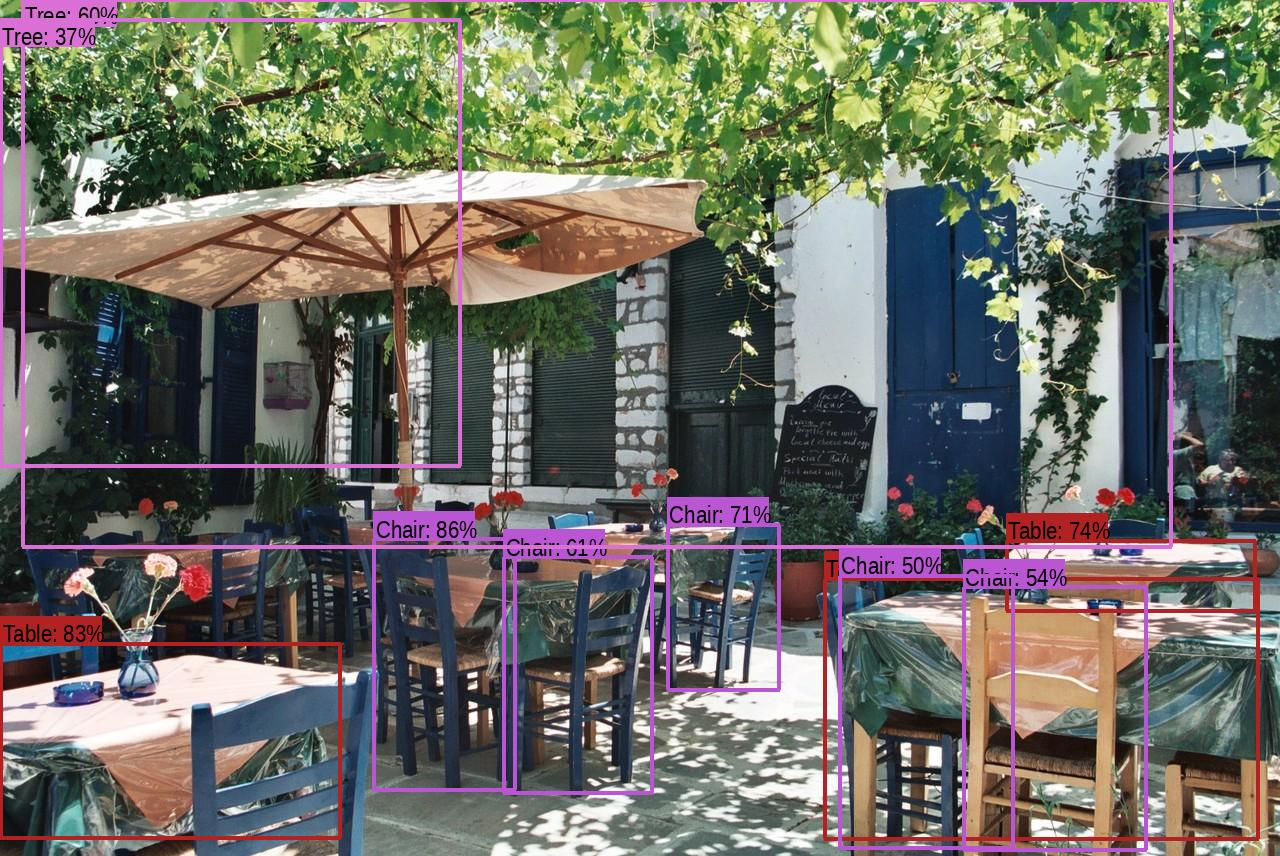
\includegraphics[scale=0.25]{../code/processed/processed.jpg}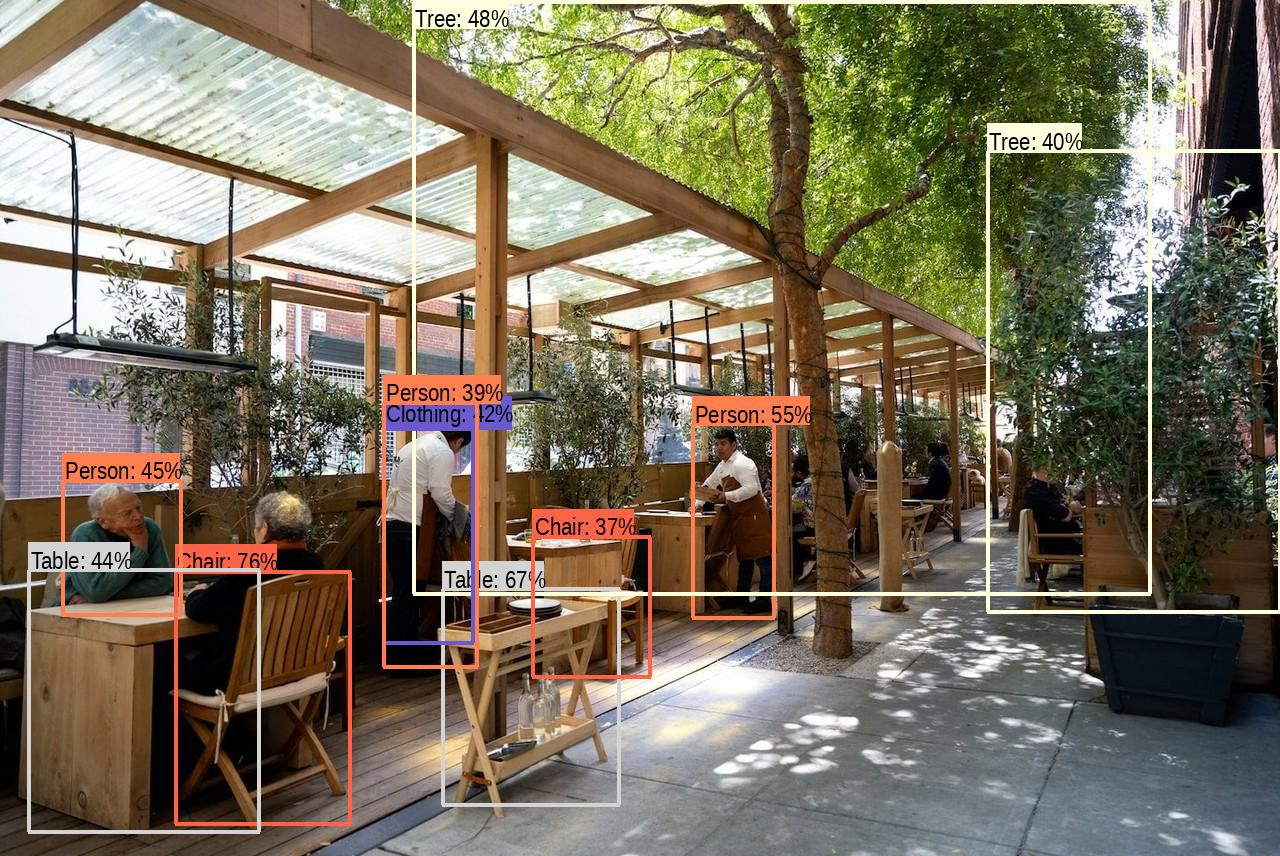
\includegraphics[scale=0.25]{../code/processed/my_image.jpg}
    \caption{Kết quả của Tensorflow API}
    \label{fig:tensor_result}
\end{figure}

\subsection{Detectron2}

\textbf{Detectron2}\cite{wu2019detectron2} là một thư viện mã nguồn mở do Facebook AI research phát triển, hỗ trợ cả hai thuật toán detection và segmentation.

Sau quá trình cài đặt thử nghiệm, nhận thấy việc cài đặt tại máy khó khăn và cần nhiều thư viện tương thích, vì vậy sử dụng notebook mẫu của Meta và thay đổi đường dẫn hình ảnh. Code được thể hiện như trong \cite{detectron2demo}.

Sử dụng hình ảnh tùy chọn tương tự ví dụ với \textit{TensorFlow}, ta được kết quả như hình \ref{fig:detection2}

\begin{figure}
    \centering
    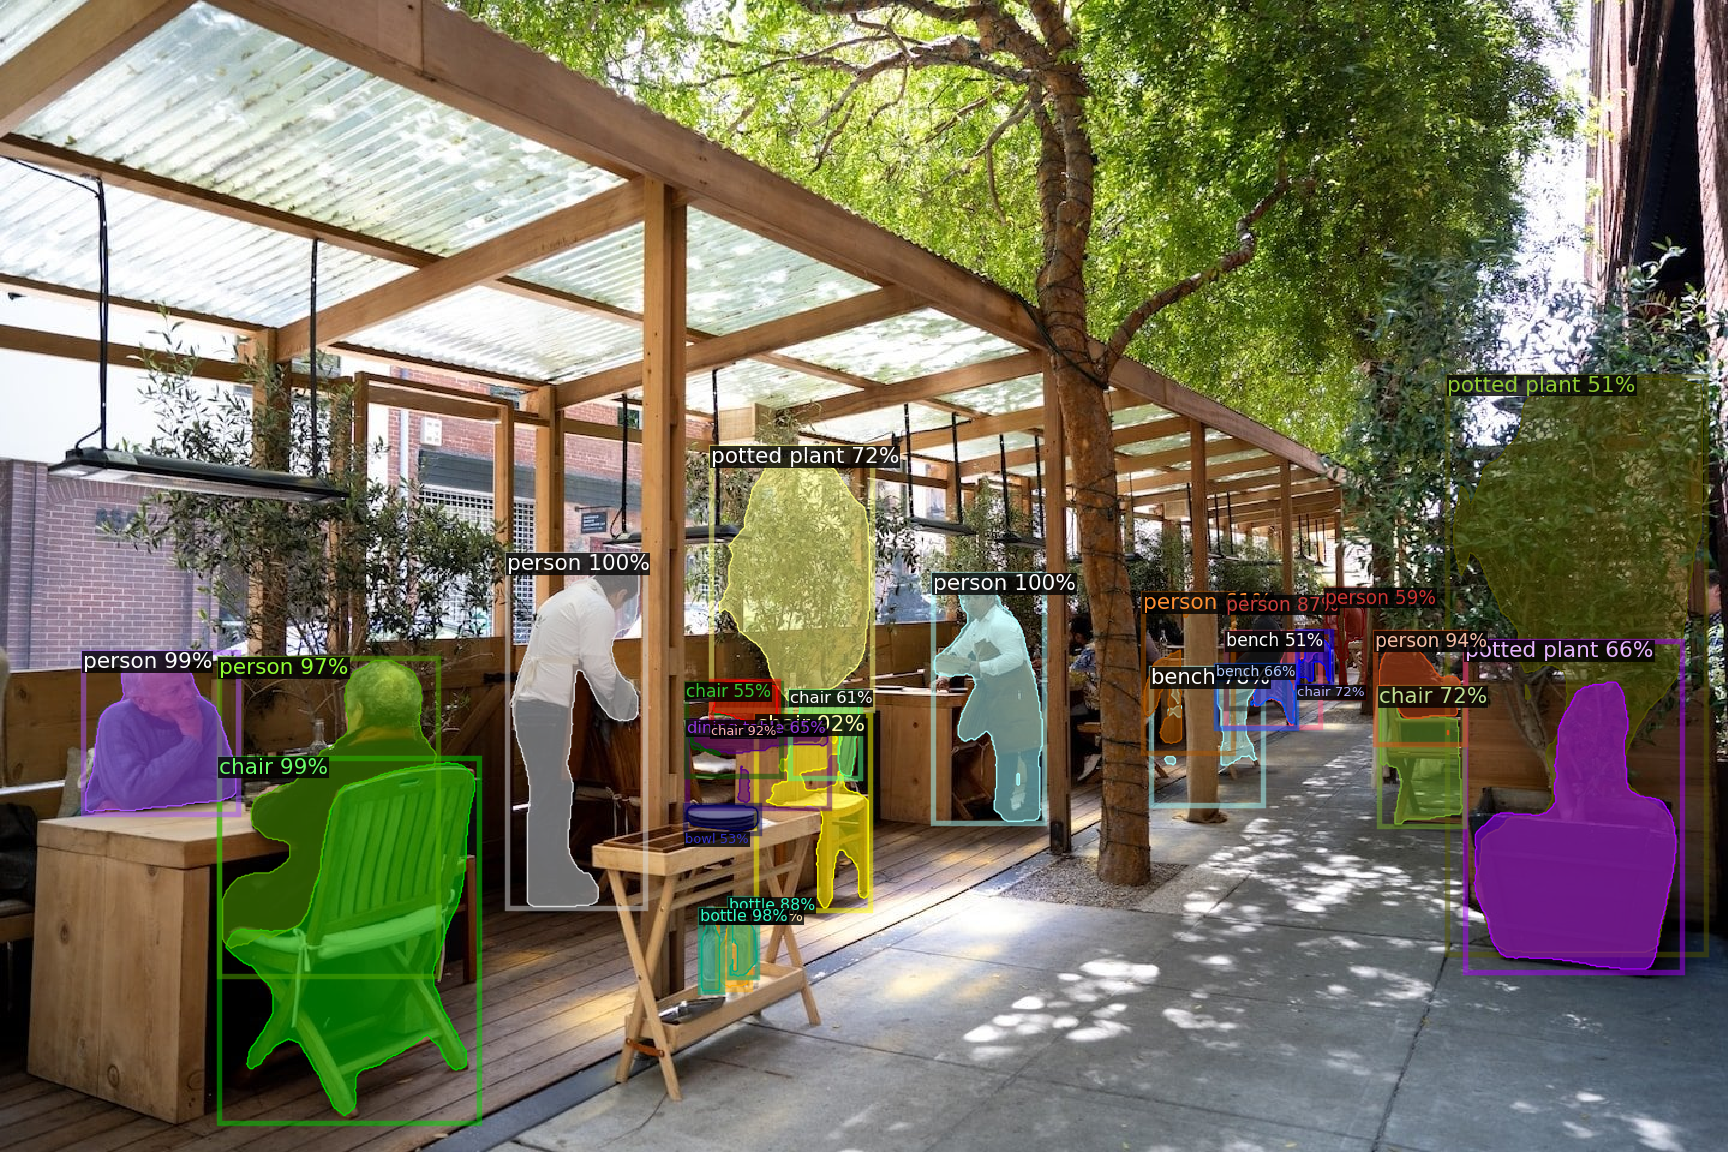
\includegraphics[scale=0.2]{../code/processed/detection2.png}
    \caption{Kết quả của Detectron2}
    \label{fig:detection2}
\end{figure}

\subsection{MXNet GluonCV}

\textbf{MXNet GluonCV} là một framework đang được phát triển bởi Apache Software Foundation \cite{apacheglucon,gluoncvnlp2020}. Nó hỗ trợ nhiều bài toán trong xử lý ảnh như Image Classification, Object Detection, Semantic Segmentation, Instance Segmentation\dots

Vì vậy, trong 

\section{Methodology}
\label{method}

\lipsum
\section{Kết luận}
\label{sec:compare}

Sau khi tìm hiểu và tiến hành thử nghiệm các thư viện, học viên nhận thấy

\begin{itemize}
    \item Về mặt chức năng và tài liệu, GluonCV nổi trội hơn cả. Nó có nhiều chức năng và tài liệu hỗ trợ, theo khuôn khổ của Apache nên cấu trúc khoa học và dễ sử dụng. Các thư viện còn lại tương tự nhau.
    \item Về mặt cài đặt, cấu hình, MMDetection là dễ cài đặt nhất. Tensor và GluonCV khó hơn do xung đột phiên bản nhưng vẫn có thể cài đặt. Còn detectron2 thì khó dùng, chỉ sử dụng trên colab.
    \item Về tốc độ inference, nhìn chung MMDetection và GluonCV khá nhanh. Detectron2 thì không thể so sánh do dùng tài nguyên của colab không giống các thư viện còn lại. Tensor thì rất lâu cho mỗi hình
\end{itemize}
\section{Implementation plan}
\label{planing}



\begingroup
\let\clearpage\relax
\printbibliography[heading=bibintoc, title = {Tài liệu tham khảo}]
\endgroup

\end{document}

